\documentclass{article}
\usepackage[T1]{fontenc}
\usepackage{lmodern}
\usepackage{graphicx}
\usepackage{amsmath,amssymb}
\usepackage[a4paper,margin=2cm]{geometry}
\usepackage[absolute,overlay]{textpos}
\setlength{\TPHorizModule}{1mm}
\setlength{\TPVertModule}{1mm}
\usepackage[indonesian]{babel}
\usepackage{hyperref}
\setlength{\emergencystretch}{2em}
% unit: Halaman 13

\begin{document}

% === Halaman 13 (python/native) ===

• Contoh lain:

13

Sumber gambar: Debdeep Mukhopadhyay, Elliptic Curve Cryptography ,

 Dept of Computer Sc and Engg IIT Madras

m = (yp – yq)/(xp – xq) 

    =(-1.86-0.836)/(-2.35-(-0.1))

    = -2.696 / -2.25 = 1.198

xr = m2 – xp – xq  

     = (1.198)2 – (-2.35) – (-0.1)

    = 3.89 

yr = m(xp – xr) – yp 

    = 1.198(-2.35 – 3.89) – (-1.86)

    = –5.62

% deskripsi: gambar native xref 71
\noindent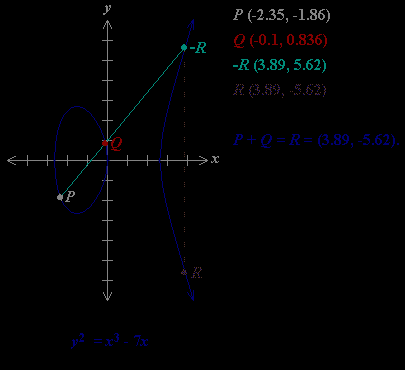
\includegraphics[width=0.85\textwidth]{../../images/python/page_013_img_01.png}

\end{document}
